\documentclass[12pt,a4paper]{article}
 
\usepackage{float}
%für feststellen der figures und tables [H] dranschreiben
\usepackage{units}
%wird so benutzt: 
%\unit[value/Zahl]{dimension/Einheit} oder 
%\unitfrac[value/Zahl]{dimension/Einheit num/Zähler}{dimension/Einheit denum/Nenner} oder
%\nicefrac[fontcommand/Schriftart]{dimension/Einheit num/Zähler}{dimension/Einheit denum/Nenner}

\usepackage{caption}
\usepackage{subcaption}

\usepackage[left=2cm,right=2cm,top=2cm,bottom=2cm]{geometry}
\usepackage[utf8]{inputenc}
\usepackage[T1]{fontenc}
\usepackage{lmodern}
\usepackage[ngerman]{babel}
\usepackage{amsmath}
\usepackage{graphicx}
 
%niemals zwei überschriften direkt übereinander schreiben, also immer mindestens in einem satz was sinnvolles unter jede überschrift schreiben (bei den versuchen z.B. das versuchsziel) 
\begin{document}
%deckblatt erstellen.


\begin{titlepage}

\begin{center}
% Oberer Teil der Titelseite:

\includegraphics[width=0.75\textwidth]{logo.pdf}\\[1cm]    	%Logo 

\textsc{\LARGE Bergische Universität Wuppertal}\\[1.5cm]	%Institution

\textsc{\Large Elektronik Praktikum}\\[0.5cm]				%Projekt


\newcommand{\HRule}{\rule{\linewidth}{0.5mm}}
\HRule \\[0.4cm]
{ \huge \bfseries Versuch EP8 Digitalelektronk Teil 1}\\[0.4cm]				%Titel

\HRule \\[1.5cm]

% Author und Tutor
\begin{minipage}{0.4\textwidth}
\begin{flushleft} \large
\emph{Autoren:}\\
Henrik \textsc{Jürgens} \\
Frederik \textsc{Strothmann}
\end{flushleft}
\end{minipage}
\hfill
\begin{minipage}{0.4\textwidth}
\begin{flushright} \large
\emph{Tutoren:} \\
Hans-Peter \textsc{Kind} \\
Peter \textsc{Knieling} \\
Marius \textsc{Wensing}
\end{flushright}
\end{minipage}

\vfill

% Unterer Teil der Seite/Datum
{\large \today}

\end{center}

\end{titlepage}

\newpage
\tableofcontents
\newpage
\section{Einleitung}
%einleitung zu dem experiment.
%auf die einstellungen, die vor dem versuch gemacht werden, eingehen oder auf eine anleitung dazu verweisen
%es soll immer erwähnt werden um was es in dem Versuch geht und wie das relisiert werden soll
%---------------------------------------------------------------------------------------------
%hinter der einleitung kann der allgemeine theoretische hintergrund in einer zusätzlichen section erklärt werden
%1-----------------------------------------------1
Die Digitaltechnik ist eine der bedeutendsten Teilgebiete der Elektronik, und wird in drei Versuche eingeteilt. Dieser Versuch beschäftigt sich mit den Grundschaltungen und einfachen Logikbausteinen. Sie findet Anwendungen in einfachen Steuerschaltungen, der Computertechnik und der heutigen Analogtechnik. Es wird zunächst das Leybold Stecksystem -- später ein Breadboard -- verwendet. 

In den einzelnen Versuchsteilen sollen die Ausgangsspannungen nach der TTL-Logik ausgewertet werden, dies geschieht nach Tabelle \ref{tab:ttl}.

\begin{table}[H]
\centering
\begin{tabular}{|l|l|}
\hline
Spannungsbereicht & Logikzustand \\ \hline
2,0 V bis 5 V & \multicolumn{1}{r|}{1} \\ \hline
0 V bis 0,8 V & \multicolumn{1}{r|}{0} \\ \hline
0,8 V bis 2 V & undefiniert \\ \hline
\end{tabular}
\caption{TTL-Logik}
\label{tab:ttl}
\end{table}


\section{Elementare Logikverknüpfungen Leybold-Stecksystem}
%kurz das ziel dieses versuchsteiles ansprechen, damit keine zwei überschriften direkt übereinander stehen!
%bei schwierigeren versuchen kann auch der theoretische hintergrund erläutert werden. (mit formeln, herleitungen und erklärungen)

In diesem Versuchsabschnitt, werden drei grundlegende logische Schaltungen mit Hilfe des Leybold-Stecksystems untersucht. Es werden die UND-, ODER- und die NICHT-Verknüpfung untersucht.

\subsection{UND-Verknüpfung}
\label{sec:UND}
%kurz das ziel dieses versuchsteiles ansprechen, damit keine zwei überschriften direkt übereinander stehen!
%bei schwierigeren versuchen kann auch der theoretische hintergrund erläutert werden. (mit formeln, herleitungen und erklärungen)

In diesem Versuchsteil wird die UND-Verknüpfung untersucht. Die UND-Verknüpfung liefert eine 1, wenn alle eingaben 1 sind, sonst 0.

\subsubsection*{Verwendete Geräte}
%(immer) eine skizze oder ein foto einfügen, die geräte/materialien !nummerieren! und z.b. eine legende dazu schreiben, besser wäre es das ganze in einem Fließtext gut zu beschreiben.
%falls am anfang des versuches nicht klar ist, was alles verwendet wird, wenn möglich erst am ende ein großes foto von den verwendeten materialien machen!\\

Es werden Widerstände, Schalter, ein Netzgerät, Dioden und ein DMM verwendet.


\subsubsection*{Versuchsaufbau}
%skizze zum versuchsaufbau (oder foto) einfügen,   es muss erklärt werden wie das ganze funktioniert und welche speziellen einstellungen verwendet wurden (z.b. welche knöpfe an den geräten für die messung verdreht wurden)

Die Werte der jeweiligen Bauteile sind der Skizze zu entnehmen.

\begin{figure}[H] 
  \centering 	
    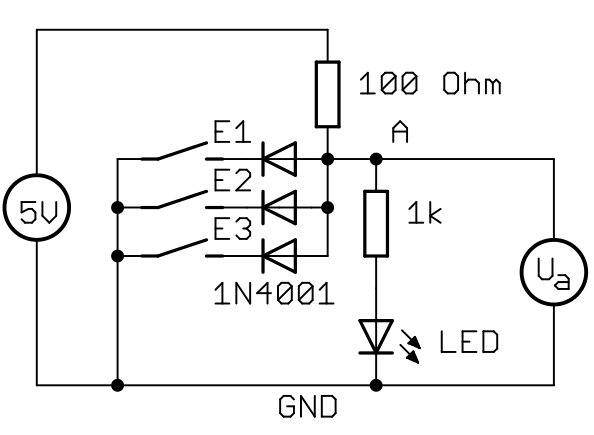
\includegraphics[ scale = 0.4]{auf_1_1.png}
  	\caption[Schaltskizze für die UND-Verknüpfung]{Schaltskizze für die UND-Verknüpfung\footnotemark}
  \label{fig:auf_1_1}
\end{figure}
\footnotetext{Abbildung entnommen von http://www.atlas.uni-wuppertal.de/$\sim$kind/ep8\_14.pdf am 13.12.2014}

\subsubsection*{Versuchsdurchführung}
%erklären, !was! wir machen, !warum! wir das machen und mit welchem ziel
%(wichtig) präzize erklären, wie bei dem versuch vorgegangen und was gemacht wurde

Die Schaltung wird nach Abbildung \ref{fig:auf_1_1} aufgebaut. Dann werden mit den Schaltern E1, E2 und E3 die Zustände in Tabelle \ref{tab:1_1} eingestellt und die Ausgangsspannung gemessen.
\subsubsection*{Auswertung}
%zuerst !alle! errechneten werte entweder in ganzen sätzen aufzählen, oder in tabellen (übersichtlicher) dargestellen, sowie auf die verwendeten formeln verweisen (die referenzierung der formel kann in der überschrift stehen)
%kurz erwähnen (vor der tabelle), warum wir das ganze ausrechnen bzw. was wir dort ausrechnen
%danach histogramme und plots erstellen, wobei wenn möglich funktionen durch die plots gelegt werden (zur not können auch splines benutzt werden, was aber angegeben werden muss)
%bei fits immer die funktion und das reduzierte chiquadrat mit angegeben, wobei auf verständlichkeit beim entziffern der zehnerpotenzen geachtet werden muss z.b. f(x)=(wert+-fehler)\cdot10^{irgendeine zahl}\cdot x + (wert+-fehler)\cdot10^{irgendeine zahl}
%bei jedem fit erklären, nach welchem zusammenhang gefittet wurde und warum!
%bei plots darauf achten, dass die achsenbeschriftung (auch die tics) die richtige größe haben und die legende im plot nicht die messwerte verdeckt
%kurz die aufgabenstellung abhandeln
%2-----------------------------------------------2

Es sollte die Ausgangsspannung gemessen werden und nach Tabelle \ref{tab:ttl} ausgewertet werde, für die verschieden Kombinationen ergab sich die Werte in Tabelle \ref{tab:1_1}.

\begin{table}[H]
\begin{center}
\begin{tabular}{r|r|r|l}

\multicolumn{1}{l|}{E1} & \multicolumn{1}{l|}{E2} & \multicolumn{1}{l|}{E3} & A \\ \hline \hline
0 & 0 & 0 & 0 \\ 
0 & 0 & 1 & 0 \\ 
0 & 1 & 0 & 0 \\ 
0 & 1 & 1 & 0 \\ 
1 & 0 & 0 & 0 \\ 
1 & 0 & 1 & 0 \\ 
1 & 1 & 0 & 0 \\ 
1 & 1 & 1 & 1 \\ 
\end{tabular}
\end{center}
\caption{Logiktabelle für die UND-Verknüpfung}
\label{tab:1_1}
\end{table}

Sobald der Ausgang auf 1 steht wird eine Spannung von 4,3 Volt gemessen. Das liegt an dem Spannungsabfall an der Diode von etwa \unit[0,7]{V}.
Offene Schalter werden in diesem Versuchsteil als logische 1 interpretiert, damit die Logiktabelle mit der 'UND-Tabelle' übereinstimmt.

\subsection{ODER-Verknüpfung}
%kurz das ziel dieses versuchsteiles ansprechen, damit keine zwei überschriften direkt übereinander stehen!
%bei schwierigeren versuchen kann auch der theoretische hintergrund erläutert werden. (mit formeln, herleitungen und erklärungen)

\label{sec:or}

In diesem Versuchsteil wird die ODER-Verknüpfung untersucht, sie gibt eine 1 wenn mindestens einer der Eingänge auf 1 gestellt ist, sonst wird 0 ausgegeben.

\subsubsection*{Verwendete Geräte}
%(immer) eine skizze oder ein foto einfügen, die geräte/materialien !nummerieren! und z.b. eine legende dazu schreiben, besser wäre es das ganze in einem Fließtext gut zu beschreiben.
%falls am anfang des versuches nicht klar ist, was alles verwendet wird, wenn möglich erst am ende ein großes foto von den verwendeten materialien machen!\\

Es werden Widerstände, Schalter, ein Netzgerät, Dioden und ein DMM verwendet.

\subsubsection*{Versuchsaufbau}
%skizze zum versuchsaufbau (oder foto) einfügen,   es muss erklärt werden wie das ganze funktioniert und welche speziellen einstellungen verwendet wurden (z.b. welche knöpfe an den geräten für die messung verdreht wurden)

Die Werte der jeweiligen Bauteile sind der Skizze zu entnehmen.

\begin{figure}[H] 
  \centering 	
    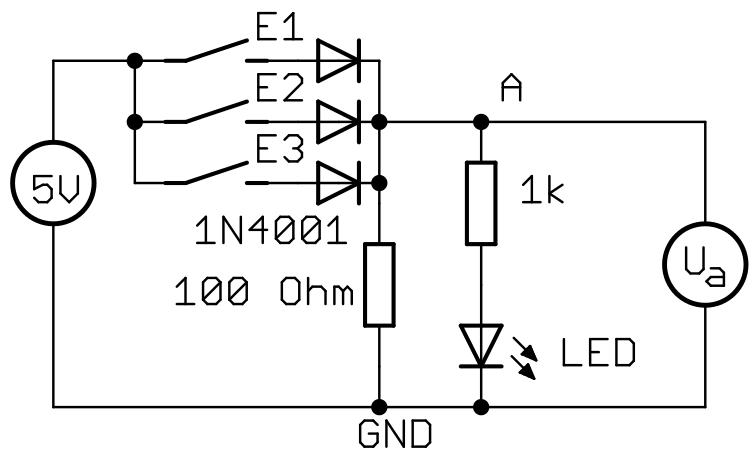
\includegraphics[ scale = 0.4]{auf_1_2.png}
  	\caption[Schaltskizze für die ODER-Verknüpfung]{Schaltskizze für die ODER-Verknüpfung\footnotemark}
  \label{fig:auf_1_2}
\end{figure}
\footnotetext{Abbildung entnommen von http://www.atlas.uni-wuppertal.de/$\sim$kind/ep8\_14.pdf am 13.12.2014}

\subsubsection*{Versuchsdurchführung}
%erklären, !was! wir machen, !warum! wir das machen und mit welchem ziel
%(wichtig) präzize erklären, wie bei dem versuch vorgegangen und was gemacht wurde

Die Schaltung in Abbildung \ref{fig:auf_1_2} wird aufgebaut. Dann werden an den Schaltern die E1, E2 und E3 die Zustände in Tabelle \ref{tab:1_2} eingestellt und die Spannung gemessen.


\subsubsection*{Auswertung}
%zuerst !alle! errechneten werte entweder in ganzen sätzen aufzählen, oder in tabellen (übersichtlicher) dargestellen, sowie auf die verwendeten formeln verweisen (die referenzierung der formel kann in der überschrift stehen)
%kurz erwähnen (vor der tabelle), warum wir das ganze ausrechnen bzw. was wir dort ausrechnen
%danach histogramme und plots erstellen, wobei wenn möglich funktionen durch die plots gelegt werden (zur not können auch splines benutzt werden, was aber angegeben werden muss)
%bei fits immer die funktion und das reduzierte chiquadrat mit angegeben, wobei auf verständlichkeit beim entziffern der zehnerpotenzen geachtet werden muss z.b. f(x)=(wert+-fehler)\cdot10^{irgendeine zahl}\cdot x + (wert+-fehler)\cdot10^{irgendeine zahl}
%bei jedem fit erklären, nach welchem zusammenhang gefittet wurde und warum!
%bei plots darauf achten, dass die achsenbeschriftung (auch die tics) die richtige größe haben und die legende im plot nicht die messwerte verdeckt
%kurz die aufgabenstellung abhandeln
%2-----------------------------------------------2


Es sollte wieder die Ausgangsspannung in Abhängigkeit der Schalterkombination gemessen und nach Tabelle \ref{tab:ttl} ausgewertet werden. Dabei ergaben sich die Werte in Tabelle \ref{tab:1_2}.

\begin{table}[H]
\begin{center}
\begin{tabular}{r|r|r|l}

\multicolumn{1}{l|}{E1} & \multicolumn{1}{l|}{E2} & \multicolumn{1}{l|}{E3} & A \\ \hline \hline
0 & 0 & 0 & 0 \\ 
0 & 0 & 1 & 1 \\ 
0 & 1 & 0 & 1 \\ 
0 & 1 & 1 & 1 \\ 
1 & 0 & 0 & 1 \\ 
1 & 0 & 1 & 1 \\ 
1 & 1 & 0 & 1 \\ 
1 & 1 & 1 & 1 \\ 
\end{tabular}
\end{center}
\caption{Logiktabelle für die ODER-Verknüpfung}
\label{tab:1_2}
\end{table}

Wie im vorigen Versuchsteil werden nicht \unit[5]{V} am Ausgang gemessen, falls er auf 1 steht, sondern etwa \unit[4,3]{V}, da ungefähr \unit[0,7]{V} an der Diode abfällt.
Geschlossene Schalter werden in diesem Versuchsteil als logische 1 interpretiert, damit die Logiktabelle der 'ODER-Tabelle' entspricht.

\subsection{NICHT-Verknüpfung}
%kurz das ziel dieses versuchsteiles ansprechen, damit keine zwei überschriften direkt übereinander stehen!
%bei schwierigeren versuchen kann auch der theoretische hintergrund erläutert werden. (mit formeln, herleitungen und erklärungen)

In diesem Versuchsteil werden die NICHT-Verknüpfung untersucht, diese liefert das Gegenteil des Eingangssignals.

\subsubsection*{Verwendete Geräte}
%(immer) eine skizze oder ein foto einfügen, die geräte/materialien !nummerieren! und z.b. eine legende dazu schreiben, besser wäre es das ganze in einem Fließtext gut zu beschreiben.
%falls am anfang des versuches nicht klar ist, was alles verwendet wird, wenn möglich erst am ende ein großes foto von den verwendeten materialien machen!\\

Es werden Widerstände, Schalter, ein Netzgerät, ein Transistor, Dioden und ein DMM verwendet.

\subsubsection*{Versuchsaufbau}
%skizze zum versuchsaufbau (oder foto) einfügen,   es muss erklärt werden wie das ganze funktioniert und welche speziellen einstellungen verwendet wurden (z.b. welche knöpfe an den geräten für die messung verdreht wurden)

Die Werte bzw. Typen der Bauteile sind der Skizze zu entnehmen.

\begin{figure}[H] 
  \centering 	
    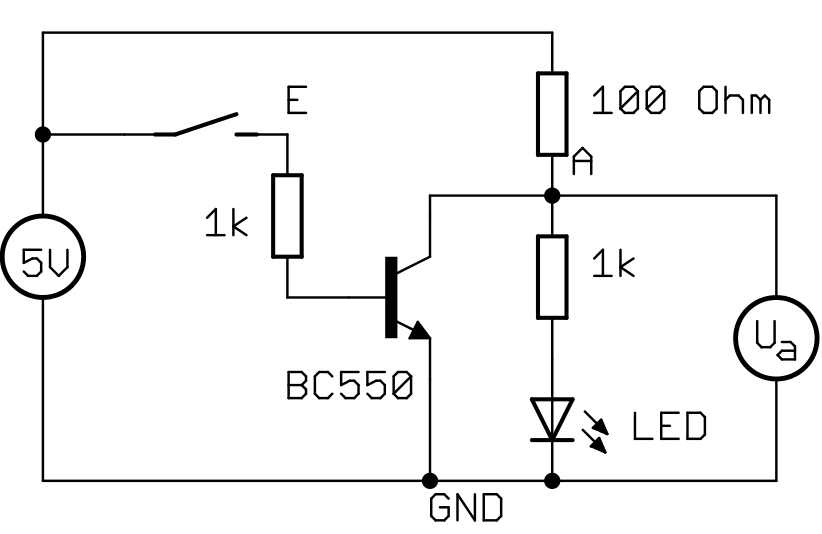
\includegraphics[ scale = 0.4]{auf_1_3.png}
  	\caption[Schaltskizze für die NICHT-Verknüpfung]{Schaltskizze für die NICHT-Verknüpfung\footnotemark}
  \label{fig:auf_1_3}
\end{figure}
\footnotetext{Abbildung entnommen von http://www.atlas.uni-wuppertal.de/$\sim$kind/ep8\_14.pdf am 13.12.2014}

\subsubsection*{Versuchsdurchführung}
%erklären, !was! wir machen, !warum! wir das machen und mit welchem ziel
%(wichtig) präzize erklären, wie bei dem versuch vorgegangen und was gemacht wurde

Die Schaltung in Abbildung \ref{fig:auf_1_3} wird aufgebaut und der Schalter nach Tabelle \ref{tab:1_3} eingestellt und die Spannung gemessen.

\subsubsection*{Auswertung}
%zuerst !alle! errechneten werte entweder in ganzen sätzen aufzählen, oder in tabellen (übersichtlicher) dargestellen, sowie auf die verwendeten formeln verweisen (die referenzierung der formel kann in der überschrift stehen)
%kurz erwähnen (vor der tabelle), warum wir das ganze ausrechnen bzw. was wir dort ausrechnen
%danach histogramme und plots erstellen, wobei wenn möglich funktionen durch die plots gelegt werden (zur not können auch splines benutzt werden, was aber angegeben werden muss)
%bei fits immer die funktion und das reduzierte chiquadrat mit angegeben, wobei auf verständlichkeit beim entziffern der zehnerpotenzen geachtet werden muss z.b. f(x)=(wert+-fehler)\cdot10^{irgendeine zahl}\cdot x + (wert+-fehler)\cdot10^{irgendeine zahl}
%bei jedem fit erklären, nach welchem zusammenhang gefittet wurde und warum!
%bei plots darauf achten, dass die achsenbeschriftung (auch die tics) die richtige größe haben und die legende im plot nicht die messwerte verdeckt
%kurz die aufgabenstellung abhandeln
%2-----------------------------------------------2

In dieser Schaltung macht es Sinn auch die Spannung über dem Schalter und GND zu messen, da über dem dahinter liegendem Transistor 0,6V abfallen, die gemessene Ausgangsspannung als kleiner ist. Es solle die Ausgangsspannung nach Tabelle \ref{tab:ttl} ausgewertet werden, das Ergebnis ist in Tabelle \ref{tab:1_3} angegeben.

\begin{table}[H]
\begin{center}
\begin{tabular}{r|l}

\multicolumn{1}{l|}{E1} & A \\ \hline \hline
0 & 1 \\ 
1 & 0 \\ 
\end{tabular}
\end{center}
\caption{Logiktabelle für die NICHT-Verknüpfung}
\label{tab:1_3}
\end{table}
Ein geschlossener Schalter wird in diesem Versuchsteil als logische 1 interpretiert.
Es wurden für das Ausgangssignal 1 \unit[4,53]{V} gemessen, also sind ca. \unit[0,47]{V} an dem \unit[100]{$\Omega$} Widerstand abgefallen.
Für das Ausgangssignal 0 wurde wurde eine Spannung von etwa \unit[0,1]{V} gemessen, also sind ca. \unit[4,9]{V} an dem \unit[100]{$\Omega$} Widerstand abgefallen.

\subsubsection*{Diskussion}
%(immer) die gemessenen werte und die bestimmten werte über die messfehler mit literaturwerten oder untereinander vergleichen
%in welchem fehlerintervall des messwertes liegt der literaturwert oder der vergleichswert?
%wie ist der relative anteil des fehlers am messwert und damit die qualität unserer messung?
%in einem satz erklären, wie gut unser fehler und damit unsere messung ist
%kurz erläutern, wie systematische fehler unsere messung beeinflusst haben könnten
%(wichtig) zum schluss ansprechen, in wie weit die ergebnisse mit der theoretischen vorhersage übereinstimmen
%--------------------------------------------------------------------------------------------
%falls tabellen mit den messwerten zu lang werden, kann die section mit den messwerten auch hinter der diskussion angefügt bzw. eine section mit dem anhang eingefügt werden.
%1-----------------------------------------------1

Alle drei Logikbausteine haben wie erwartet funktioniert, wobei die Interpretation der Schalterstellung von der UND auf die ODER-Verknüpfung abgeändert werden musste. Bei der UND-Schaltung wurden offene Schalter als logische 1 interpretiert, wobei in der ODER-Scahltung geschlossene Schalter als logische 1 interpretiert wurden. 

\section{Elementare Logikverknüpfungen ICs und Breadboard}
%kurz das ziel dieses versuchsteiles ansprechen, damit keine zwei überschriften direkt übereinander stehen!
%bei schwierigeren versuchen kann auch der theoretische hintergrund erläutert werden. (mit formeln, herleitungen und erklärungen)

In diesem Versuchsabschnitt werde ICs untersucht, da dies 14 bis 16 Pins haben ist der Aufbau für das Leybold-Stecksystem zu groß und es werden Breadboards verwendet. Es werden NAND-, AND- und OR-Verknüpfungen mit dem IC untersucht. Danach werden Inverter, Schmitt-Trigger, das RS-Flipflop, das Zählflipflop und eine Ziffernanzeige mit Siebensegmentdecoder untersucht. Der in diesem Versuch hauptsächlich verwendet IC besteht aus vier NAND-Verknüpfungen (Pin 1-6 und 8-13) und zwei Pins für die Spannungsversorgung (Pin 7 und 14). Falls nicht anders angegeben entspricht ein offener Schalter einer 0 und ein geschlossener Schalter einer 1.

\subsection{NICHT-UND-Verknüpfung (NAND)}
%kurz das ziel dieses versuchsteiles ansprechen, damit keine zwei überschriften direkt übereinander stehen!
%bei schwierigeren versuchen kann auch der theoretische hintergrund erläutert werden. (mit formeln, herleitungen und erklärungen)

In diesem Versuchsteil wird die NAND-Verknüpfung untersucht. Die NAND-Verknüpfung entspricht der Negation der AND-Verknüpfung (siehe Abschnitt \ref{sec:UND}).

\subsubsection*{Verwendete Geräte}
%(immer) eine skizze oder ein foto einfügen, die geräte/materialien !nummerieren! und z.b. eine legende dazu schreiben, besser wäre es das ganze in einem Fließtext gut zu beschreiben.
%falls am anfang des versuches nicht klar ist, was alles verwendet wird, wenn möglich erst am ende ein großes foto von den verwendeten materialien machen!\\

Es werden ein Netzgerät, ein IC, Widerstände, ein Diode und Schalter verwendet.

\subsubsection*{Versuchsaufbau}
%skizze zum versuchsaufbau (oder foto) einfügen,   es muss erklärt werden wie das ganze funktioniert und welche speziellen einstellungen verwendet wurden (z.b. welche knöpfe an den geräten für die messung verdreht wurden)

R1 und R2 sind die beiden Pulldown-Widerstände mit jeweils 10k$\Omega$. R3 ist ein 1k$\Omega$ Widerstand.

\begin{figure}[H] 
  \centering 	
    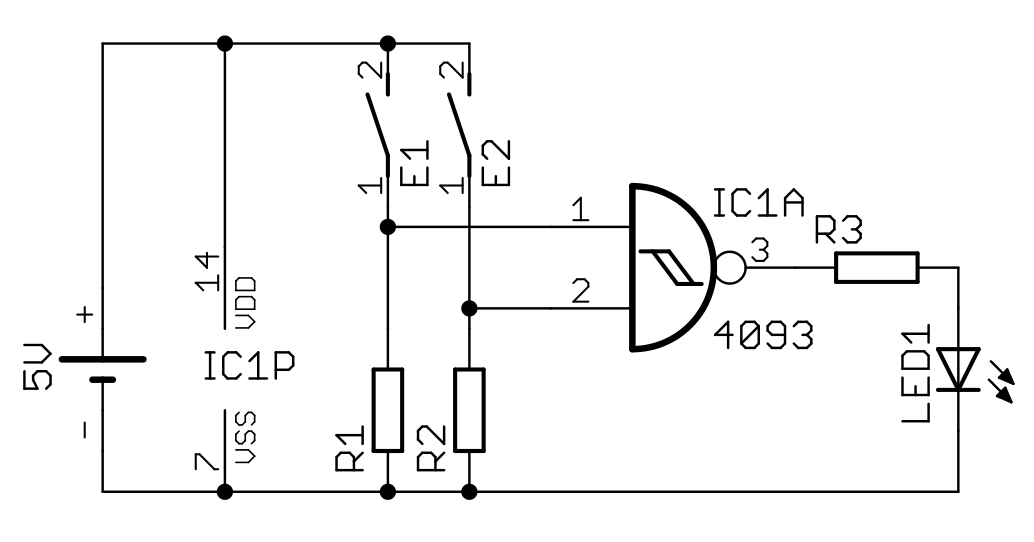
\includegraphics[ scale = 0.4]{auf_2_1.png}
  	\caption[Schaltskizze für die NAND-Verknüpfung]{Schaltskizze für die NAND-Verknüpfung\footnotemark}
  \label{fig:auf_2_1}
\end{figure}
\footnotetext{Abbildung entnommen von http://www.atlas.uni-wuppertal.de/$\sim$kind/ep8\_14.pdf am 13.12.2014}

\subsubsection*{Versuchsdurchführung}
%erklären, !was! wir machen, !warum! wir das machen und mit welchem ziel
%(wichtig) präzize erklären, wie bei dem versuch vorgegangen und was gemacht wurde

Die Schaltung wird nach Abbildung \ref{fig:auf_2_1} aufgebaut. Dann werden an den Schaltern die Kombinationen nach Tabelle \ref{tab:2_1} eingestellt und das Verhalten der LED ausgewertet.

\subsubsection*{Auswertung}
%zuerst !alle! errechneten werte entweder in ganzen sätzen aufzählen, oder in tabellen (übersichtlicher) dargestellen, sowie auf die verwendeten formeln verweisen (die referenzierung der formel kann in der überschrift stehen)
%kurz erwähnen (vor der tabelle), warum wir das ganze ausrechnen bzw. was wir dort ausrechnen
%danach histogramme und plots erstellen, wobei wenn möglich funktionen durch die plots gelegt werden (zur not können auch splines benutzt werden, was aber angegeben werden muss)
%bei fits immer die funktion und das reduzierte chiquadrat mit angegeben, wobei auf verständlichkeit beim entziffern der zehnerpotenzen geachtet werden muss z.b. f(x)=(wert+-fehler)\cdot10^{irgendeine zahl}\cdot x + (wert+-fehler)\cdot10^{irgendeine zahl}
%bei jedem fit erklären, nach welchem zusammenhang gefittet wurde und warum!
%bei plots darauf achten, dass die achsenbeschriftung (auch die tics) die richtige größe haben und die legende im plot nicht die messwerte verdeckt
%kurz die aufgabenstellung abhandeln
%2-----------------------------------------------2

Es sollte die NAND-Verknüpfung des ICs untersucht werden, es ergaben sich dabei die Werte in Tabelle \ref{tab:2_1}.

\begin{table}[H]
\begin{center}
\begin{tabular}{r|r|l}

\multicolumn{1}{l|}{E1} & \multicolumn{1}{l|}{E2} & A \\ \hline \hline
0 & 0 & 1 \\ 
0 & 1 & 1 \\ 
1 & 0 & 1 \\ 
1 & 1 & 0 \\ 
\end{tabular}
\end{center}
\caption{Logiktabelle für die NAND-Verknüpfung}
\label{tab:2_1}
\end{table}


\subsubsection*{Diskussion}
%(immer) die gemessenen werte und die bestimmten werte über die messfehler mit literaturwerten oder untereinander vergleichen
%in welchem fehlerintervall des messwertes liegt der literaturwert oder der vergleichswert?
%wie ist der relative anteil des fehlers am messwert und damit die qualität unserer messung?
%in einem satz erklären, wie gut unser fehler und damit unsere messung ist
%kurz erläutern, wie systematische fehler unsere messung beeinflusst haben könnten
%(wichtig) zum schluss ansprechen, in wie weit die ergebnisse mit der theoretischen vorhersage übereinstimmen
%--------------------------------------------------------------------------------------------
%falls tabellen mit den messwerten zu lang werden, kann die section mit den messwerten auch hinter der diskussion angefügt bzw. eine section mit dem anhang eingefügt werden.
%1-----------------------------------------------1
Wie erwartet konnten die Eigenschaften der NAND-Tabelle festgestellt werden. Die Schaltung hat erst nach zweimaligem Neuaufbau funktioniert, was an den sehr kleinen Anschlüssen gelegen haben kann.(Wackelkontakte)
\subsection{UND-Verknüpfung (AND)}
%kurz das ziel dieses versuchsteiles ansprechen, damit keine zwei überschriften direkt übereinander stehen!
%bei schwierigeren versuchen kann auch der theoretische hintergrund erläutert werden. (mit formeln, herleitungen und erklärungen)

In diesem Versuchsteil wird die AND-Verknüpfung über zwei NAND-Verknüpfungen realisiert. Das Verhalten der AND-Verknüpfung ist in Abschnitt \ref{sec:UND} erklärt.

\subsubsection*{Verwendete Geräte}
%(immer) eine skizze oder ein foto einfügen, die geräte/materialien !nummerieren! und z.b. eine legende dazu schreiben, besser wäre es das ganze in einem Fließtext gut zu beschreiben.
%falls am anfang des versuches nicht klar ist, was alles verwendet wird, wenn möglich erst am ende ein großes foto von den verwendeten materialien machen!\\

Es werden ein Netzgerät, ein IC, Widerstände, ein Diode und Schalter verwendet.


\subsubsection*{Versuchsaufbau}
%skizze zum versuchsaufbau (oder foto) einfügen,   es muss erklärt werden wie das ganze funktioniert und welche speziellen einstellungen verwendet wurden (z.b. welche knöpfe an den geräten für die messung verdreht wurden)

R1 und R2 sind die beiden Pulldown-Widerstände mit jeweils 10k$\Omega$. R3 ist ein 1k$\Omega$ Widerstand.

\begin{figure}[H] 
  \centering 	
    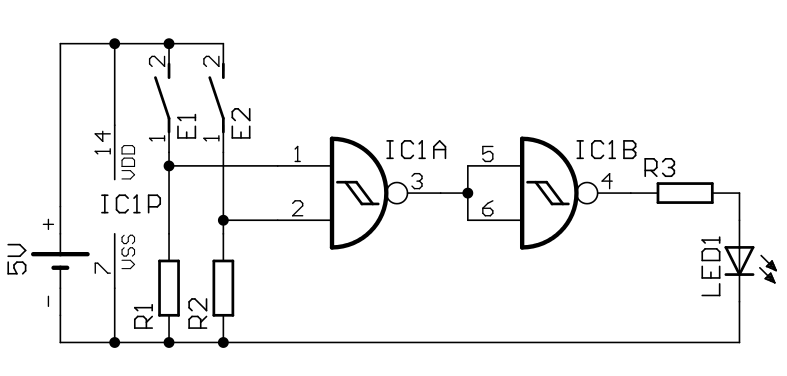
\includegraphics[ scale = 0.4]{auf_2_2.png}
  	\caption[Schaltskizze für die UND-Verknüpfung]{Schaltskizze für die UND-Verknüpfung\footnotemark}
  \label{fig:auf_2_2}
\end{figure}
\footnotetext{Abbildung entnommen von http://www.atlas.uni-wuppertal.de/$\sim$kind/ep8\_14.pdf am 13.12.2014}

\subsubsection*{Versuchsdurchführung}
%erklären, !was! wir machen, !warum! wir das machen und mit welchem ziel
%(wichtig) präzize erklären, wie bei dem versuch vorgegangen und was gemacht wurde

Die Schaltung wird nach Abbildung \ref{fig:auf_2_2} aufgebaut. Dann werden die Schalter nach Tabelle \ref{tab:2_2} eingestellt und das Verhalten der LED beobachtet.

\subsubsection*{Auswertung}
%zuerst !alle! errechneten werte entweder in ganzen sätzen aufzählen, oder in tabellen (übersichtlicher) dargestellen, sowie auf die verwendeten formeln verweisen (die referenzierung der formel kann in der überschrift stehen)
%kurz erwähnen (vor der tabelle), warum wir das ganze ausrechnen bzw. was wir dort ausrechnen
%danach histogramme und plots erstellen, wobei wenn möglich funktionen durch die plots gelegt werden (zur not können auch splines benutzt werden, was aber angegeben werden muss)
%bei fits immer die funktion und das reduzierte chiquadrat mit angegeben, wobei auf verständlichkeit beim entziffern der zehnerpotenzen geachtet werden muss z.b. f(x)=(wert+-fehler)\cdot10^{irgendeine zahl}\cdot x + (wert+-fehler)\cdot10^{irgendeine zahl}
%bei jedem fit erklären, nach welchem zusammenhang gefittet wurde und warum!
%bei plots darauf achten, dass die achsenbeschriftung (auch die tics) die richtige größe haben und die legende im plot nicht die messwerte verdeckt
%kurz die aufgabenstellung abhandeln
%2-----------------------------------------------2

Es soll das Verhalten der UND-Verknüpfung aus zwei hintereinander geschalteten NAND-Verknüpfungen untersucht werden, dabei ergeben sich für die LED die Werte in Tabelle \ref{tab:2_2}.

\begin{table}[H]
\begin{center}
\begin{tabular}{r|r|l}

\multicolumn{1}{l|}{E1} & \multicolumn{1}{l|}{E2} & A \\ \hline \hline
0 & 0 & 0 \\ 
0 & 1 & 0 \\ 
1 & 0 & 0 \\ 
1 & 1 & 1 \\ 
\end{tabular}
\end{center}
\caption{Logiktabelle für die AND-Verknüpfung}
\label{tab:2_2}
\end{table}


\subsubsection*{Diskussion}
%(immer) die gemessenen werte und die bestimmten werte über die messfehler mit literaturwerten oder untereinander vergleichen
%in welchem fehlerintervall des messwertes liegt der literaturwert oder der vergleichswert?
%wie ist der relative anteil des fehlers am messwert und damit die qualität unserer messung?
%in einem satz erklären, wie gut unser fehler und damit unsere messung ist
%kurz erläutern, wie systematische fehler unsere messung beeinflusst haben könnten
%(wichtig) zum schluss ansprechen, in wie weit die ergebnisse mit der theoretischen vorhersage übereinstimmen
%--------------------------------------------------------------------------------------------
%falls tabellen mit den messwerten zu lang werden, kann die section mit den messwerten auch hinter der diskussion angefügt bzw. eine section mit dem anhang eingefügt werden.
%1-----------------------------------------------1

Es ergaben sich jeweils die erwarteten Werte bei den verschiedenen Kombinationen.

\subsection{ODER-Verknüpfung (OR)}
%kurz das ziel dieses versuchsteiles ansprechen, damit keine zwei überschriften direkt übereinander stehen!
%bei schwierigeren versuchen kann auch der theoretische hintergrund erläutert werden. (mit formeln, herleitungen und erklärungen)

In diesem Versuchsteil soll die OR-Verknüpfung bestehend aus 3 NAND-Verknüpfungen untersucht werden. Die Funktionsweise einer OR-Verknüpfung wird in Abschnitt \ref{sec:or} erklärt.

\subsubsection*{Verwendete Geräte}
%(immer) eine skizze oder ein foto einfügen, die geräte/materialien !nummerieren! und z.b. eine legende dazu schreiben, besser wäre es das ganze in einem Fließtext gut zu beschreiben.
%falls am anfang des versuches nicht klar ist, was alles verwendet wird, wenn möglich erst am ende ein großes foto von den verwendeten materialien machen!\\

Es werden ein Netzgerät, ein IC, Widerstände, ein Diode und Schalter verwendet.


\subsubsection*{Versuchsaufbau}
%skizze zum versuchsaufbau (oder foto) einfügen,   es muss erklärt werden wie das ganze funktioniert und welche speziellen einstellungen verwendet wurden (z.b. welche knöpfe an den geräten für die messung verdreht wurden)

R1 und R2 sind die beiden Pulldown-Widerstände mit jeweils 10k$\Omega$. R3 ist ein 1k$\Omega$ Widerstand.

\begin{figure}[H] 
  \centering 	
    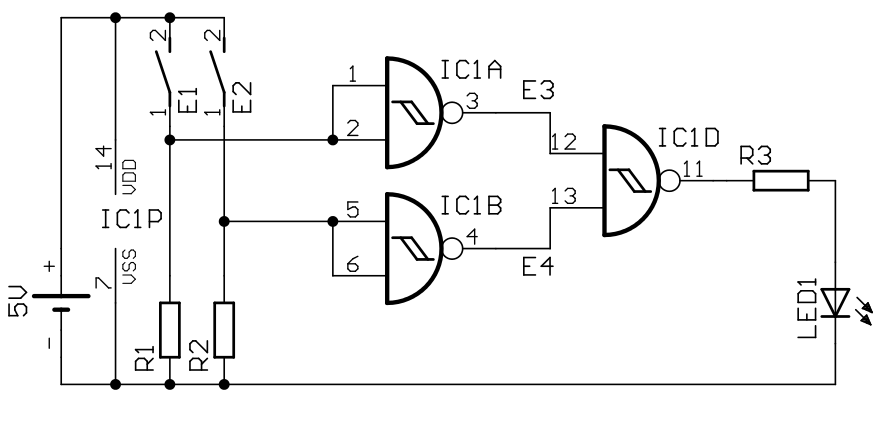
\includegraphics[ scale = 0.4]{auf_2_3.png}
  	\caption[Schaltskizze für die OR-Verknüpfung]{Schaltskizze für die OR-Verknüpfung\footnotemark}
  \label{fig:auf_2_3}
\end{figure}
\footnotetext{Abbildung entnommen von http://www.atlas.uni-wuppertal.de/$\sim$kind/ep8\_14.pdf am 13.12.2014}

\subsubsection*{Versuchsdurchführung}
%erklären, !was! wir machen, !warum! wir das machen und mit welchem ziel
%(wichtig) präzize erklären, wie bei dem versuch vorgegangen und was gemacht wurde

Die Schaltung wird nach Abbildung \ref{fig:auf_2_3} aufgebaut. Die Schalter werden dann nach Tabelle \ref{tab:2_3} eingestellt und das Verhalten der LED beobachtet.

\subsubsection*{Auswertung}
%zuerst !alle! errechneten werte entweder in ganzen sätzen aufzählen, oder in tabellen (übersichtlicher) dargestellen, sowie auf die verwendeten formeln verweisen (die referenzierung der formel kann in der überschrift stehen)
%kurz erwähnen (vor der tabelle), warum wir das ganze ausrechnen bzw. was wir dort ausrechnen
%danach histogramme und plots erstellen, wobei wenn möglich funktionen durch die plots gelegt werden (zur not können auch splines benutzt werden, was aber angegeben werden muss)
%bei fits immer die funktion und das reduzierte chiquadrat mit angegeben, wobei auf verständlichkeit beim entziffern der zehnerpotenzen geachtet werden muss z.b. f(x)=(wert+-fehler)\cdot10^{irgendeine zahl}\cdot x + (wert+-fehler)\cdot10^{irgendeine zahl}
%bei jedem fit erklären, nach welchem zusammenhang gefittet wurde und warum!
%bei plots darauf achten, dass die achsenbeschriftung (auch die tics) die richtige größe haben und die legende im plot nicht die messwerte verdeckt
%kurz die aufgabenstellung abhandeln
%2-----------------------------------------------2

Es soll das Verhalten der OR-Verknüpfung untersucht werden. Dabei ergaben sich die Werte in Tabelle \ref{fig:auf_2_3}.

\begin{table}[H]
\begin{center}
\begin{tabular}{r|r|r|r|l}

\multicolumn{1}{l|}{E1} & \multicolumn{1}{l|}{E2} & \multicolumn{1}{l|}{E3} & \multicolumn{1}{l|}{E4} & A \\ \hline \hline
0 & 0 & 1 & 1 & 0 \\ 
0 & 1 & 1 & 0 & 1 \\ 
1 & 0 & 0 & 1 & 1 \\ 
1 & 1 & 0 & 0 & 1 \\ 
\end{tabular}
\end{center}
\caption{Logiktabelle für die ODER-Verknüpfung}
\label{tab:2_3}
\end{table}

Die ODER-Verknüpfung besteht aus drei NAND-Verknüpfungen wie in Abb. \ref{fig:auf_2_3} zu sehen ist. Zwei dieser NANDs werden in dieser Schaltung als Inverter verwendet.

\subsubsection*{Diskussion}
%(immer) die gemessenen werte und die bestimmten werte über die messfehler mit literaturwerten oder untereinander vergleichen
%in welchem fehlerintervall des messwertes liegt der literaturwert oder der vergleichswert?
%wie ist der relative anteil des fehlers am messwert und damit die qualität unserer messung?
%in einem satz erklären, wie gut unser fehler und damit unsere messung ist
%kurz erläutern, wie systematische fehler unsere messung beeinflusst haben könnten
%(wichtig) zum schluss ansprechen, in wie weit die ergebnisse mit der theoretischen vorhersage übereinstimmen
%--------------------------------------------------------------------------------------------
%falls tabellen mit den messwerten zu lang werden, kann die section mit den messwerten auch hinter der diskussion angefügt bzw. eine section mit dem anhang eingefügt werden.
%1-----------------------------------------------1

Wie erwartet konnte die Logiktabelle einer NAND-Verknüpfung gemessen werden.

\subsection{Inverter und Schmitt-Trigger}
%kurz das ziel dieses versuchsteiles ansprechen, damit keine zwei überschriften direkt übereinander stehen!
%bei schwierigeren versuchen kann auch der theoretische hintergrund erläutert werden. (mit formeln, herleitungen und erklärungen)

In diesem Versuchsteil werden der Inverter und der Schmitt-Trigger untersucht bzw. die Verwendung der beiden als Rechteckgenerator. Mit dem Schmitt-Trigger lassen sich Störungen des Eingangssignals abschneiden.

\subsubsection*{Verwendete Geräte}
%(immer) eine skizze oder ein foto einfügen, die geräte/materialien !nummerieren! und z.b. eine legende dazu schreiben, besser wäre es das ganze in einem Fließtext gut zu beschreiben.
%falls am anfang des versuches nicht klar ist, was alles verwendet wird, wenn möglich erst am ende ein großes foto von den verwendeten materialien machen!\\

Es werden ein Netzgerät, ein Kondensator, Widerstände, ein DMM, ein IC und eine LED verwendet.


\subsubsection*{Versuchsaufbau}
%skizze zum versuchsaufbau (oder foto) einfügen,   es muss erklärt werden wie das ganze funktioniert und welche speziellen einstellungen verwendet wurden (z.b. welche knöpfe an den geräten für die messung verdreht wurden)

R ist ein 1k$\Omega$ Widerstand, R1 ist ein 10k$\Omega$ Widerstand.

\begin{figure}[H] 
  \centering 	
    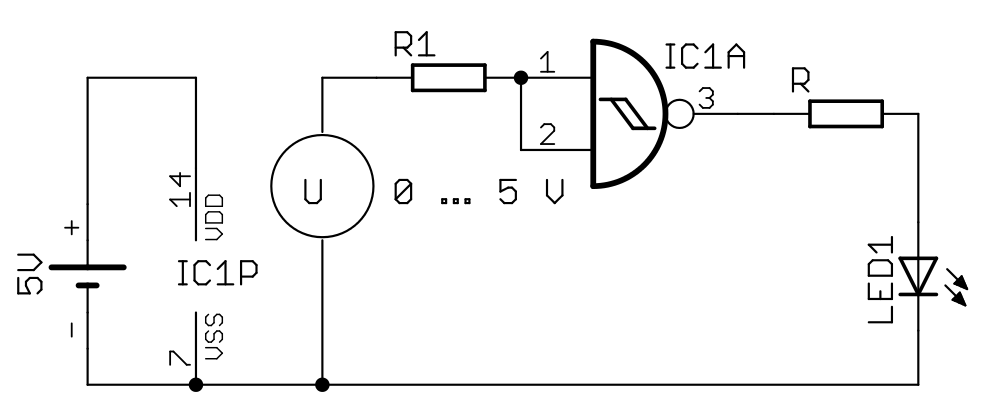
\includegraphics[ scale = 0.4]{auf_2_4_1.png}
  	\caption[Schaltskizze für den Inverter]{Schaltskizze für den Inverter\footnotemark}
  \label{fig:auf_2_4_1}
\end{figure}
\footnotetext{Abbildung entnommen von http://www.atlas.uni-wuppertal.de/$\sim$kind/ep8\_14.pdf am 13.12.2014}

R ist ein 1k$\Omega$ Widerstand, R1 ist ein 100k$\Omega$ Widerstand und C ein 10$\mu$F Kondensator.

\begin{figure}[H] 
  \centering 	
    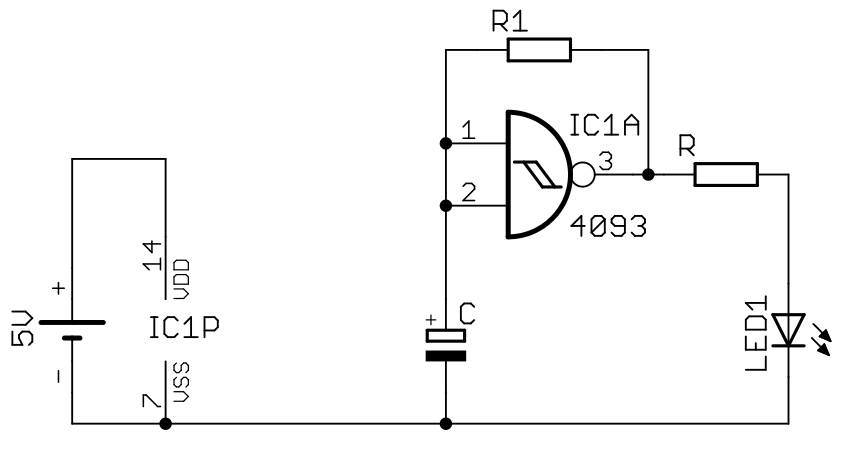
\includegraphics[ scale = 0.4]{auf_2_4_2.png}
  	\caption[Schaltskizze für den Schmitt-Trigger]{Schaltskizze für den Schmitt-Trigger\footnotemark}
  \label{fig:auf_2_4_2}
\end{figure}
\footnotetext{Abbildung entnommen von http://www.atlas.uni-wuppertal.de/$\sim$kind/ep8\_14.pdf am 13.12.2014}


\subsubsection*{Versuchsdurchführung}
%erklären, !was! wir machen, !warum! wir das machen und mit welchem ziel
%(wichtig) präzize erklären, wie bei dem versuch vorgegangen und was gemacht wurde

Die Schaltung wird nach Abbildung \ref{fig:auf_2_4_1} aufgebaut. Dann wird eine Eingangsspannung von 0V angelegt, diese wird langsam erhöht, bis die LED leuchtet und dann die Spannung gemessen. Dann wird die Spannung solange abgesenkt, bis die LED ausgeht, dann wird wieder die Spannung gemessen.

Dann wird die Schaltung aus Abbildung \ref{fig:auf_2_4_2} aufgebaut. Dann soll der 2000$\Omega$ Lautsprecher angeschlossen werden um das Signal zu untersuchen. Es soll untersucht werden bis zu welcher Frequenz die Schaltung zuverlässig funktioniert, dies geschieht durch variierten von R1 und C.

\subsubsection*{Auswertung}
%zuerst !alle! errechneten werte entweder in ganzen sätzen aufzählen, oder in tabellen (übersichtlicher) dargestellen, sowie auf die verwendeten formeln verweisen (die referenzierung der formel kann in der überschrift stehen)
%kurz erwähnen (vor der tabelle), warum wir das ganze ausrechnen bzw. was wir dort ausrechnen
%danach histogramme und plots erstellen, wobei wenn möglich funktionen durch die plots gelegt werden (zur not können auch splines benutzt werden, was aber angegeben werden muss)
%bei fits immer die funktion und das reduzierte chiquadrat mit angegeben, wobei auf verständlichkeit beim entziffern der zehnerpotenzen geachtet werden muss z.b. f(x)=(wert+-fehler)\cdot10^{irgendeine zahl}\cdot x + (wert+-fehler)\cdot10^{irgendeine zahl}
%bei jedem fit erklären, nach welchem zusammenhang gefittet wurde und warum!
%bei plots darauf achten, dass die achsenbeschriftung (auch die tics) die richtige größe haben und die legende im plot nicht die messwerte verdeckt
%kurz die aufgabenstellung abhandeln
%2-----------------------------------------------2
In der Schaltung in Abb. \ref{fig:auf_2_4_1} geht die Diode ab einer Spannung von \unit[3]{V} aus. Ab einer Spannung von \unit[2,3]{V} geht sie wieder an. Der Hysteresespiel beträgt daher etwa \unit[0,7]{V}.\newline
Im zweiten Teil soll die Schaltung aus Abb. \ref{fig:auf_2_4_2}, welche einen Rechteckgenerator darstellt aufgebaut werden. Diese Schaltung stellt deshalb einen Rechteckgenerator da, weil der Kondensator, solange der Ausgang des NAND auf 1 steht, aufgeladen wird, bis die beiden Eingänge des NAND\footnote{an denen die gleiche Spannung abfällt wie am Kondensator} aufgrund der Kondensatorspannung auf 1 schalten. Dadurch wird der Kondensator langsam entladen. Sobald die beiden Eingänge des NAND aufgrund der niedrigen Kondensatorspannung auf 0 schalten, ändert sich der Ausgang wieder auf 1 und der Vorgang beginnt von neuem. Deshalb wird Abhängig von der Kapazität und der Größe des Widerstandes eine bestimmte Frequenz erzeugt. Gemessen wurden Frequenzen von ca. \unit[1,8]{Hz} bei \unit[80,6]{k$\Omega$} \footnote{\unit[10]{$\mu$F} Kondensatorkapazität} und ca. \unit[0,18]{Hz} bei \unit[40,2]{k$\Omega$} \footnote{\unit[100]{$\mu$F} Kondensatorkapazität}.
\subsubsection*{Diskussion}
%(immer) die gemessenen werte und die bestimmten werte über die messfehler mit literaturwerten oder untereinander vergleichen
%in welchem fehlerintervall des messwertes liegt der literaturwert oder der vergleichswert?
%wie ist der relative anteil des fehlers am messwert und damit die qualität unserer messung?
%in einem satz erklären, wie gut unser fehler und damit unsere messung ist
%kurz erläutern, wie systematische fehler unsere messung beeinflusst haben könnten
%(wichtig) zum schluss ansprechen, in wie weit die ergebnisse mit der theoretischen vorhersage übereinstimmen
%--------------------------------------------------------------------------------------------
%falls tabellen mit den messwerten zu lang werden, kann die section mit den messwerten auch hinter der diskussion angefügt bzw. eine section mit dem anhang eingefügt werden.
%1-----------------------------------------------1



\subsection{Speicherbausteine: Das RS-Flipflop}
%kurz das ziel dieses versuchsteiles ansprechen, damit keine zwei überschriften direkt übereinander stehen!
%bei schwierigeren versuchen kann auch der theoretische hintergrund erläutert werden. (mit formeln, herleitungen und erklärungen)

In diesem Versuchsteil wird das RS-Flipflop untersucht. Das RS-Flipflop ist ein Speicherelement, welches aus zwei NAND-Verknüpfungen besteht.

\subsubsection*{Verwendete Geräte}
%(immer) eine skizze oder ein foto einfügen, die geräte/materialien !nummerieren! und z.b. eine legende dazu schreiben, besser wäre es das ganze in einem Fließtext gut zu beschreiben.
%falls am anfang des versuches nicht klar ist, was alles verwendet wird, wenn möglich erst am ende ein großes foto von den verwendeten materialien machen!\\
Es werden ein Netzgerät, 4 Widerstände, ein IC-Baustein 4093, zwei LEDs und zwei Schalter verwendet.
\subsubsection*{Versuchsaufbau}
%skizze zum versuchsaufbau (oder foto) einfügen,   es muss erklärt werden wie das ganze funktioniert und welche speziellen einstellungen verwendet wurden (z.b. welche knöpfe an den geräten für die messung verdreht wurden)

\begin{figure}[H] 
  \centering 	
    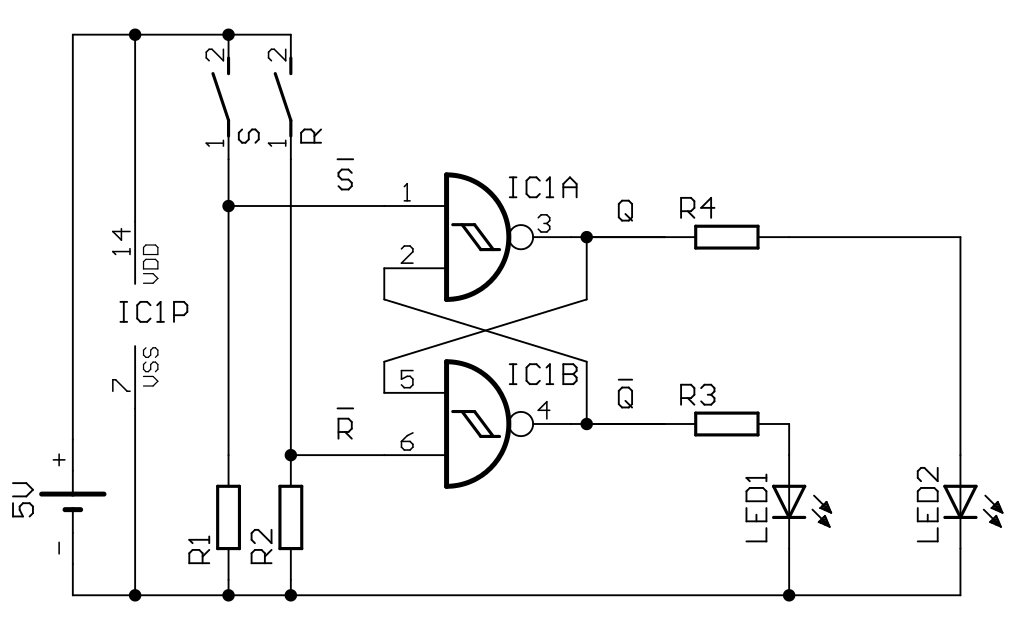
\includegraphics[ scale = 0.4]{auf_2_5.png}
  	\caption[Schaltskizze für das RS-Flipflop]{Schaltskizze für das RS-Flipflop\footnotemark}
  \label{fig:auf_2_5}
\end{figure}
\footnotetext{Abbildung entnommen von http://www.atlas.uni-wuppertal.de/$\sim$kind/ep8\_14.pdf am 13.12.2014}
Die Spannungsquelle wird auf \unit[5]{V} eingestellt, die Widerstände R1 und R2 betragen \unit[10]{k$\Omega$}, R3 und R4 betragen \unit[1]{k$\Omega$}, der IC-Baustein 4093 besteht aus 4 NAND-Gattern. Zwei LEDs und zwei Schalter sind ebenfalls verbaut.
\subsubsection*{Versuchsdurchführung}
%erklären, !was! wir machen, !warum! wir das machen und mit welchem ziel
%(wichtig) präzize erklären, wie bei dem versuch vorgegangen und was gemacht wurde
Das RS-Flipflop wird nach Abb. \ref{fig:auf_2_5} aufgebaut und die Versorgungsspannung eingeschaltet. Die Wahrheitstabelle für das RS-Flipflop wird dann durch ein bzw. ausschalten der beiden Schalter R und S aufgenommen.
\subsubsection*{Auswertung}
%zuerst !alle! errechneten werte entweder in ganzen sätzen aufzählen, oder in tabellen (übersichtlicher) dargestellen, sowie auf die verwendeten formeln verweisen (die referenzierung der formel kann in der überschrift stehen)
%kurz erwähnen (vor der tabelle), warum wir das ganze ausrechnen bzw. was wir dort ausrechnen
%danach histogramme und plots erstellen, wobei wenn möglich funktionen durch die plots gelegt werden (zur not können auch splines benutzt werden, was aber angegeben werden muss)
%bei fits immer die funktion und das reduzierte chiquadrat mit angegeben, wobei auf verständlichkeit beim entziffern der zehnerpotenzen geachtet werden muss z.b. f(x)=(wert+-fehler)\cdot10^{irgendeine zahl}\cdot x + (wert+-fehler)\cdot10^{irgendeine zahl}
%bei jedem fit erklären, nach welchem zusammenhang gefittet wurde und warum!
%bei plots darauf achten, dass die achsenbeschriftung (auch die tics) die richtige größe haben und die legende im plot nicht die messwerte verdeckt
%kurz die aufgabenstellung abhandeln
%2-----------------------------------------------2

Es sollte von dem Grundzustand (erste Zeile in Tabelle \ref{tab:2_5}) aus der Speicherzustand verändert werden und die Zustände der LEDs notiert werden. Die Ergebnisse der Messung sind in Tabelle \ref{tab:2_5} angegeben.


\begin{table}[H]
\begin{center}
\begin{tabular}{r|r|l|l}

\multicolumn{1}{l|}{$\bar{R}$} & \multicolumn{1}{l|}{$\bar{S}$} & Q & $\bar{Q}$ \\ \hline \hline
1 & 1 & \multicolumn{1}{r|}{0} & \multicolumn{1}{r}{1} \\ 
1 & 0 & 1 & 0 \\ 
1 & 1 & 1 & 0 \\ 
0 & 1 & 0 & 1 \\ 
1 & 1 & 0 & 1 \\ 
1 & 0 & 1 & 0 \\ 
1 & 1 & 1 & 0 \\ 
\end{tabular}
\end{center}
\caption{Logiktabelle für das RS-Flipflop}
\label{tab:2_5}
\end{table}

Ändert man die Schaltung wie in Abbildung \ref{fig:_2_5_2} um so kann man mit der Schaltung 1-Impuls Änderungen speichern.

\begin{figure}[H] 
  \centering 	
    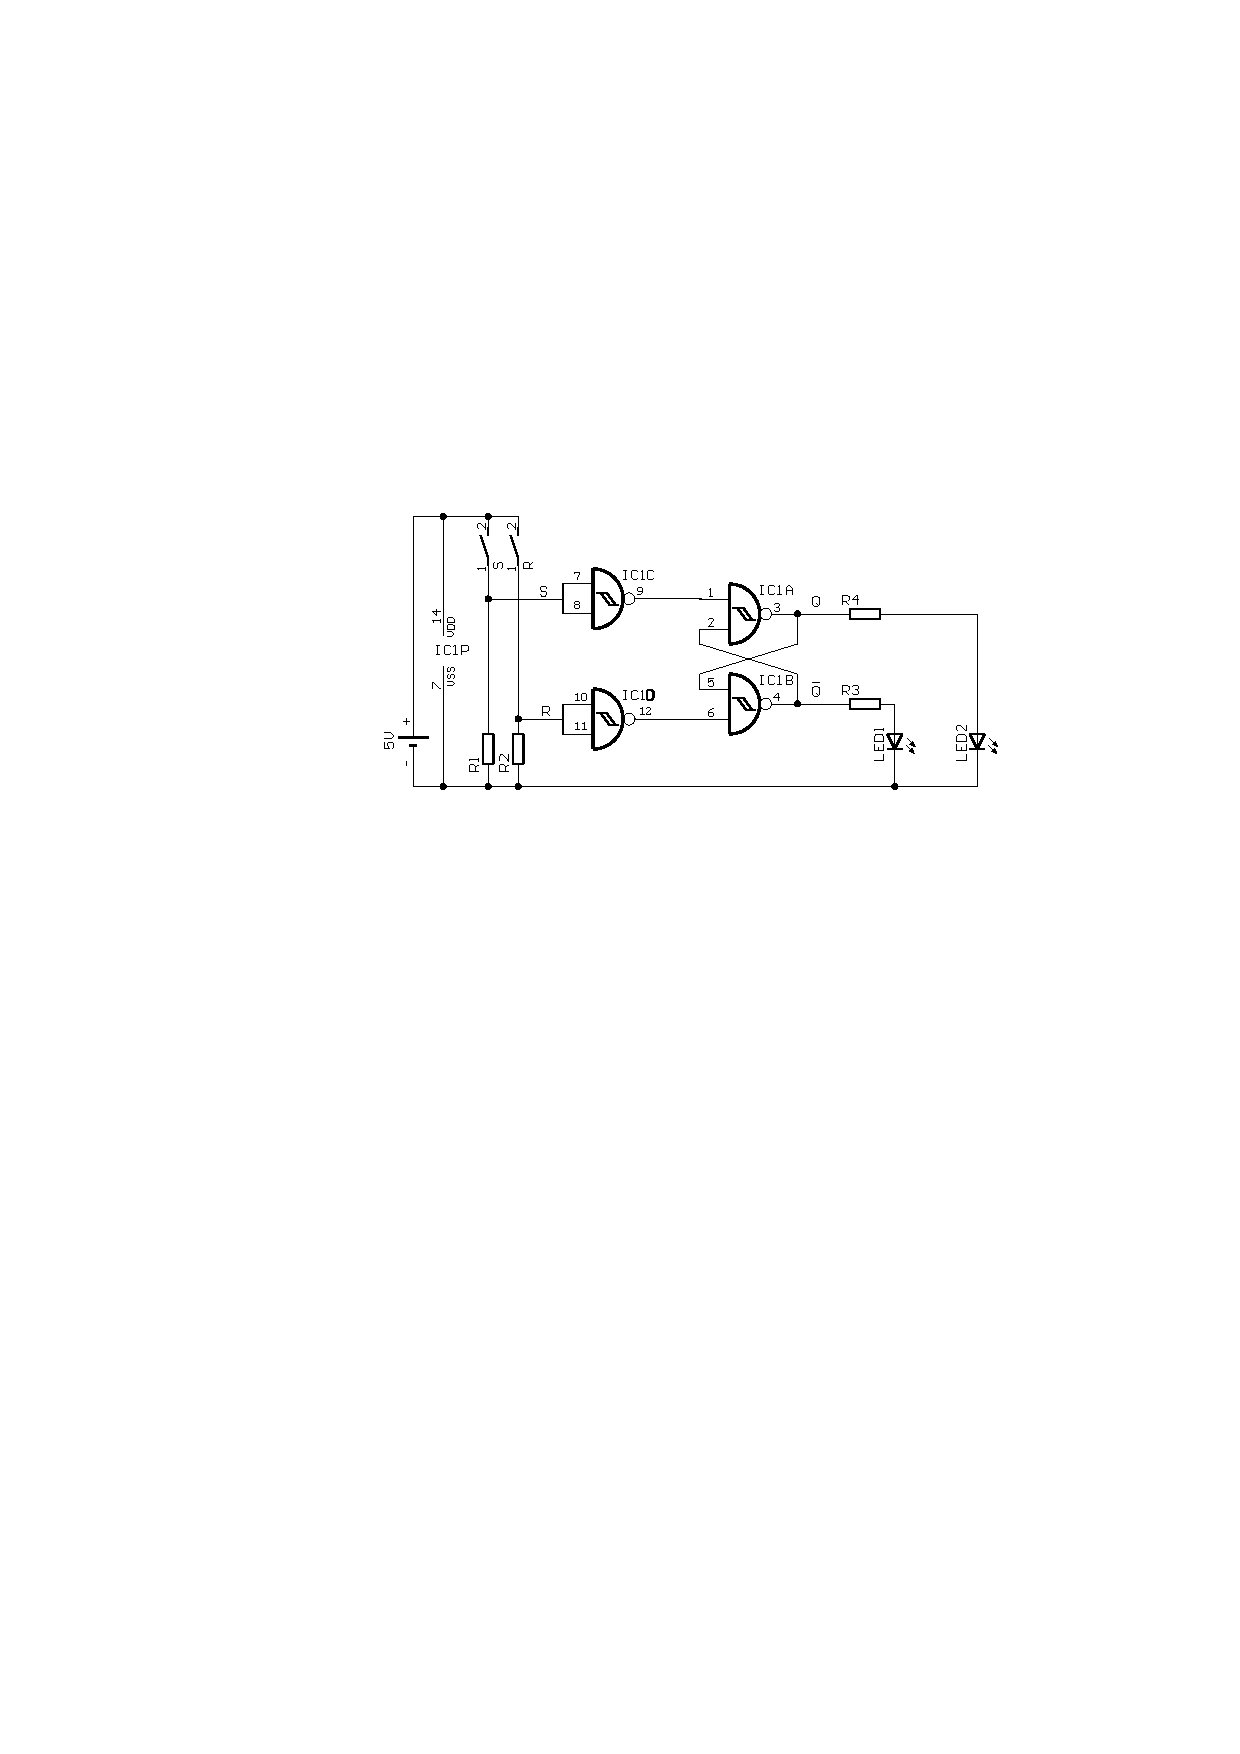
\includegraphics[ scale = 1]{2_5_2.pdf}
  	\caption[Schaltskizze zum speichern von 1-Impuls Änderungen]{Schaltskizze zum speichern von 1-Impuls Änderungen\footnotemark}
  \label{fig:_2_5_2}
\end{figure}


\subsubsection*{Diskussion}
%(immer) die gemessenen werte und die bestimmten werte über die messfehler mit literaturwerten oder untereinander vergleichen
%in welchem fehlerintervall des messwertes liegt der literaturwert oder der vergleichswert?
%wie ist der relative anteil des fehlers am messwert und damit die qualität unserer messung?
%in einem satz erklären, wie gut unser fehler und damit unsere messung ist
%kurz erläutern, wie systematische fehler unsere messung beeinflusst haben könnten
%(wichtig) zum schluss ansprechen, in wie weit die ergebnisse mit der theoretischen vorhersage übereinstimmen
%--------------------------------------------------------------------------------------------
%falls tabellen mit den messwerten zu lang werden, kann die section mit den messwerten auch hinter der diskussion angefügt bzw. eine section mit dem anhang eingefügt werden.
%1-----------------------------------------------1

Die Schaltung verhielt sich wie nach der Theorie erwartet wurde.

\subsection{Das Zähl-Flipflop}
%kurz das ziel dieses versuchsteiles ansprechen, damit keine zwei überschriften direkt übereinander stehen!
%bei schwierigeren versuchen kann auch der theoretische hintergrund erläutert werden. (mit formeln, herleitungen und erklärungen)
In diesem Versuchsteil wird das Zählflipflop untersucht, welches aus einzelnen T-Flipflops besteht.
\subsubsection*{Verwendete Geräte}
%(immer) eine skizze oder ein foto einfügen, die geräte/materialien !nummerieren! und z.b. eine legende dazu schreiben, besser wäre es das ganze in einem Fließtext gut zu beschreiben.
%falls am anfang des versuches nicht klar ist, was alles verwendet wird, wenn möglich erst am ende ein großes foto von den verwendeten materialien machen!\\
Es werden ein Netzgerät, der IC-Baustein 4040 und 4093, 9 LEDs, ein Kondensator und 10 Widerstände verwendet.


\subsubsection*{Versuchsaufbau}
%skizze zum versuchsaufbau (oder foto) einfügen,   es muss erklärt werden wie das ganze funktioniert und welche speziellen einstellungen verwendet wurden (z.b. welche knöpfe an den geräten für die messung verdreht wurden)

\begin{figure}[H] 
  \centering 	
    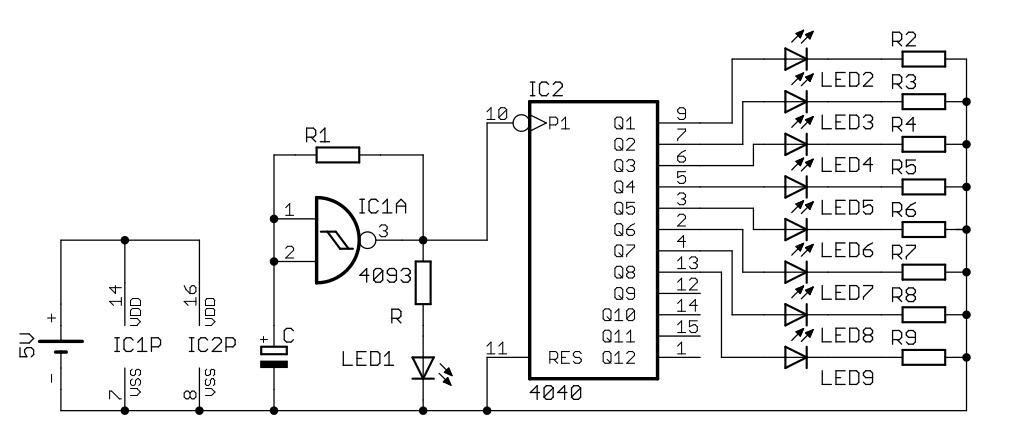
\includegraphics[ scale = 0.4]{auf_2_6.png}
  	\caption[Schaltskizze für das Zähl-Flipflop]{Schaltskizze für das Zähl-Flipflop\footnotemark}
  \label{fig:auf_2_6}
\end{figure}
\footnotetext{Abbildung entnommen von http://www.atlas.uni-wuppertal.de/$\sim$kind/ep8\_14.pdf am 13.12.2014}
Die Spannung der Spannungsquelle beträgt \unit[5]{V}, der IC-Baustein 4040 besteht aus 12 Zählflipflops, ein \unit[10]{$\mu$F} Kondensator, 8 \unit[330]{$\Omega$}, ein \unit[10]{k$\Omega$}, und ein \unit[1]{k$\Omega$} Widerstand und 9 LEDs verwendet.
\subsubsection*{Versuchsdurchführung}
%erklären, !was! wir machen, !warum! wir das machen und mit welchem ziel
%(wichtig) präzize erklären, wie bei dem versuch vorgegangen und was gemacht wurde
Es wird die Schaltung nach Abb. \ref{fig:auf_2_6} aufgebaut und der Strom eingeschaltet. Die Dioden sollten nacheinander aufblinken und im Binärsystem hochzählen. Dazu soll beobachtet werden, wie das Frequenzverhältnis bei zwei nebeneinander liegenden Dioden ist. Dann werden der Kondensator und der Widerstand R1 verändert, um die Frequenz zu verändern. Es wird wieder das Verhalten anhand der LED-Leiste untersucht.
\subsubsection*{Auswertung}
%zuerst !alle! errechneten werte entweder in ganzen sätzen aufzählen, oder in tabellen (übersichtlicher) dargestellen, sowie auf die verwendeten formeln verweisen (die referenzierung der formel kann in der überschrift stehen)
%kurz erwähnen (vor der tabelle), warum wir das ganze ausrechnen bzw. was wir dort ausrechnen
%danach histogramme und plots erstellen, wobei wenn möglich funktionen durch die plots gelegt werden (zur not können auch splines benutzt werden, was aber angegeben werden muss)
%bei fits immer die funktion und das reduzierte chiquadrat mit angegeben, wobei auf verständlichkeit beim entziffern der zehnerpotenzen geachtet werden muss z.b. f(x)=(wert+-fehler)\cdot10^{irgendeine zahl}\cdot x + (wert+-fehler)\cdot10^{irgendeine zahl}
%bei jedem fit erklären, nach welchem zusammenhang gefittet wurde und warum!
%bei plots darauf achten, dass die achsenbeschriftung (auch die tics) die richtige größe haben und die legende im plot nicht die messwerte verdeckt
%kurz die aufgabenstellung abhandeln
%2-----------------------------------------------2
Auf der LED-Leiste wurde die einzelnen LEDs von links nach rechts aufgefüllt, wenn die nächste rechte LED erreicht wurde, wurden die vorherigen abgeschaltet und es fing der nächste zähl Durchlauf bis zur nächsten LED an.
Es wurde beobachtet, dass die jeweils nächste Stufe immer mit der Hälfte der Frequenz der Stufe davor blinkt. D.h. das Frequenzverhältnis zwischen zwei nebeneinander liegenden Dioden beträgt immer eine Oktave.
\subsubsection*{Diskussion}
%(immer) die gemessenen werte und die bestimmten werte über die messfehler mit literaturwerten oder untereinander vergleichen
%in welchem fehlerintervall des messwertes liegt der literaturwert oder der vergleichswert?
%wie ist der relative anteil des fehlers am messwert und damit die qualität unserer messung?
%in einem satz erklären, wie gut unser fehler und damit unsere messung ist
%kurz erläutern, wie systematische fehler unsere messung beeinflusst haben könnten
%(wichtig) zum schluss ansprechen, in wie weit die ergebnisse mit der theoretischen vorhersage übereinstimmen
%--------------------------------------------------------------------------------------------
%falls tabellen mit den messwerten zu lang werden, kann die section mit den messwerten auch hinter der diskussion angefügt bzw. eine section mit dem anhang eingefügt werden.
%1-----------------------------------------------1



\subsection{Ziffernanzeige Siebensegmentdecoder 4511}
%kurz das ziel dieses versuchsteiles ansprechen, damit keine zwei überschriften direkt übereinander stehen!
%bei schwierigeren versuchen kann auch der theoretische hintergrund erläutert werden. (mit formeln, herleitungen und erklärungen)

In diesem Versuchsteil wird die Siebensegmentanzeige und ein Siebensegmentdecoder untersucht. Mit den Bauteilen aus den vorangegangenen Versuchsteilen wird auf der Siebensegmentanzeige die Zahlen von 0 bis 9 durchgezählt.

\subsubsection*{Verwendete Geräte}
%(immer) eine skizze oder ein foto einfügen, die geräte/materialien !nummerieren! und z.b. eine legende dazu schreiben, besser wäre es das ganze in einem Fließtext gut zu beschreiben.
%falls am anfang des versuches nicht klar ist, was alles verwendet wird, wenn möglich erst am ende ein großes foto von den verwendeten materialien machen!\\

Es werden ein ICs des Typs 4040, 4093 und 4511, Widerstände, eine Siebensegmentanzeige, ein Netzgerät, ein Kondensator und Dioden verwendet. 


\subsubsection*{Versuchsaufbau}
%skizze zum versuchsaufbau (oder foto) einfügen,   es muss erklärt werden wie das ganze funktioniert und welche speziellen einstellungen verwendet wurden (z.b. welche knöpfe an den geräten für die messung verdreht wurden)

C ist ein 10$\mu$F Kondensator, R und R2 bis R9 sind 1k$\Omega$ Widerstände. 

\begin{figure}[H] 
  \centering 	
    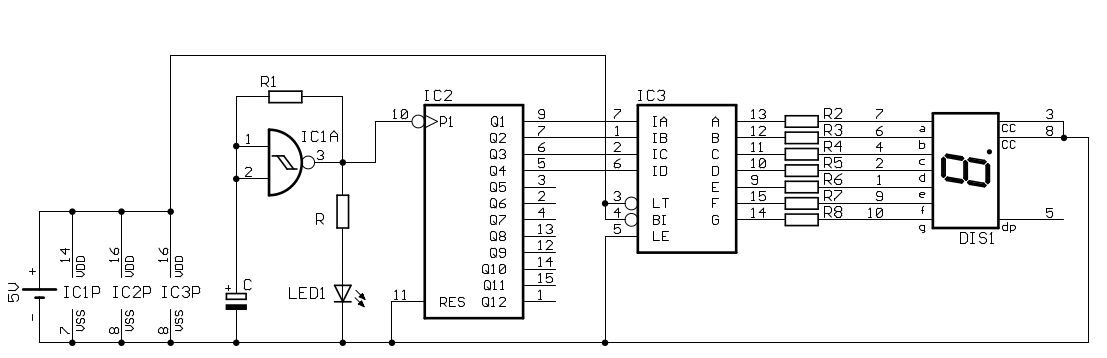
\includegraphics[ scale = 0.4]{auf_2_7.png}
  	\caption[Schaltskizze für die Siebensegmentanzeige, ohne Reset beim erreichten von 10]{Schaltskizze für die Siebensegmentanzeige, ohne Reset beim erreichten von 10\footnotemark}
  \label{fig:auf_2_7}
\end{figure}
\footnotetext{Abbildung entnommen von http://www.atlas.uni-wuppertal.de/$\sim$kind/ep8\_14.pdf am 13.12.2014}

C ist ein 10$\mu$F Kondensator, R und R2 bis R9 sind 1k$\Omega$ Widerstände.

\begin{figure}[H] 
  \centering 	
    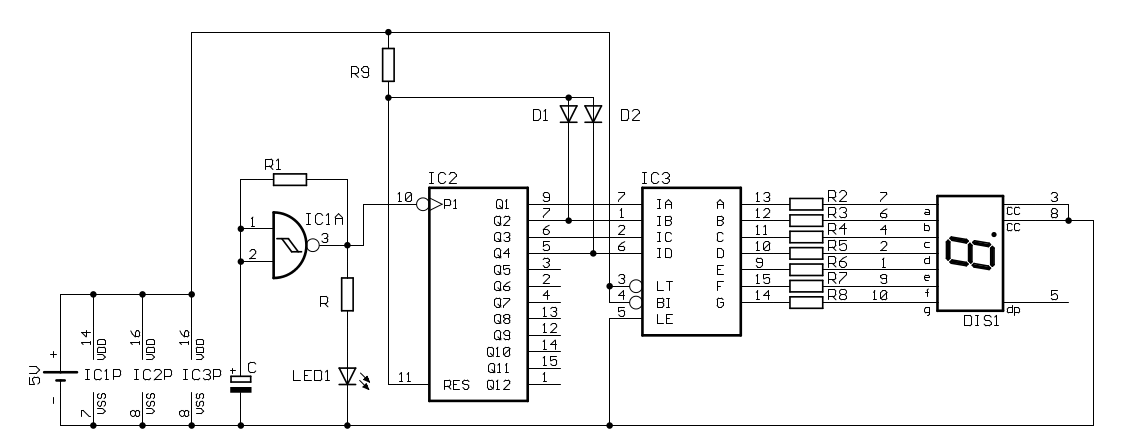
\includegraphics[ scale = 0.4]{auf_2_7_2.png}
  	\caption[Schaltskizze für die Siebensegmentanzeige, mit Reset beim erreichten von 10]{Schaltskizze für die Siebensegmentanzeige, mit Reset beim erreichten von 10\footnotemark}
  \label{fig:auf_2_7_2}
\end{figure}
\footnotetext{Abbildung entnommen von http://www.atlas.uni-wuppertal.de/$\sim$kind/ep8\_14.pdf am 13.12.2014}

\subsubsection*{Versuchsdurchführung}
%erklären, !was! wir machen, !warum! wir das machen und mit welchem ziel
%(wichtig) präzize erklären, wie bei dem versuch vorgegangen und was gemacht wurde
Die Schaltung des Siebensegmentdecoders wird nach Abb. \ref{fig:auf_2_7} aufgebaut und die Spannungsversorgung eingeschaltet. Das aufleuchten der LEDs des Siebensegmentdecoders kann dann beobachtet werden. Der Siebensegmentdecoder sollte von 1 bis 9 hochzählen.

\subsubsection*{Auswertung}
%zuerst !alle! errechneten werte entweder in ganzen sätzen aufzählen, oder in tabellen (übersichtlicher) dargestellen, sowie auf die verwendeten formeln verweisen (die referenzierung der formel kann in der überschrift stehen)
%kurz erwähnen (vor der tabelle), warum wir das ganze ausrechnen bzw. was wir dort ausrechnen
%danach histogramme und plots erstellen, wobei wenn möglich funktionen durch die plots gelegt werden (zur not können auch splines benutzt werden, was aber angegeben werden muss)
%bei fits immer die funktion und das reduzierte chiquadrat mit angegeben, wobei auf verständlichkeit beim entziffern der zehnerpotenzen geachtet werden muss z.b. f(x)=(wert+-fehler)\cdot10^{irgendeine zahl}\cdot x + (wert+-fehler)\cdot10^{irgendeine zahl}
%bei jedem fit erklären, nach welchem zusammenhang gefittet wurde und warum!
%bei plots darauf achten, dass die achsenbeschriftung (auch die tics) die richtige größe haben und die legende im plot nicht die messwerte verdeckt
%kurz die aufgabenstellung abhandeln
%2-----------------------------------------------2

Im ersten Aufbau (Abbildung \ref{fig:auf_2_7}) konnte wie erwartet das Durchzählen von 0 bis 9 mit kurzer Pause vor dem Neuanfang beobachtet werden. In der Verbesserten Schaltung (Abbildung \ref{fig:auf_2_7_2}) entfiel die Pause nach 9, da durch die Sperrung der Leitungen für 8 und 2 der Resetschalter mit Spannung versorgt wurde. Dieser Vorgang geschieht so schnell, dass er nicht wahrnehmbar ist und es einem so Vorkommt, dass nach 9 sofort bei 0 wieder angefangen wird.


\section{Fazit}
%im fazit nochmal alles zusammenfassen und den verlauf der messung abschätzen
%gravierende sytematische probleme bei den messungen nochmal betonen und die wertigkeit unserer ergebnisse einordnen
\end{document}

